\section{Andmestiku loomine}
Selles peatükis käsitletakse andmestiku loomise protsessi, sealhulgas andmete kogumist, töötlemist ja maskimist. Andmestiku loomine on oluline samm igasuguste andmete analüüsimisel ja seda ka masinõppe projektide puhul. Andmete kvaliteet ja sobivus mõjutavad otseselt mudeli täpsust ja usaldusväärsust. Nagu muudes valdkondades kehtib ka informaatikas Pareto printsiip, mille kohaselt 80\% probleemidest tuleneb 20\% põhjustest. Seega on andmestiku loomine ja töötlemine äärmiselt oluline etapp, mis võib määrata kogu projekti edasise käigu.

\subsection{Raie piirkonna andmete kogumine}
Metsateatis on dokument, mille kaudu metsaomanik esitab Keskkonnaametile
kavandatavate raietööde või oluliste metsakahjustuste kohta teabe. Keskkonnaamet
kontrollib esitatud teatiste nõuetekohasust ning veendub, et kavandatav raie
vastab kehtivatele õigusaktidele. Metsateatised menetletakse ja säilitatakse
riiklikus metsaregistris. Peale edukat menetlemist võib raietöödega alustada 10 päeva peale otsust ja kuni 24 kuu jooksul. \cite{MetsateatisJaMetsaregister} Metsateatised on avalikud ja neid saab vaadata riiklikus metsaregistris.

Metsade inventeerimise ja registrisse kandmise protsess algab metsaeraldiste
täpse kaardistamisega, kasutades L‑EST97 ristkoordinaatide süsteemi, Eesti
põhikaarti, katastriüksuse plaane ning vajadusel kaugseire andmeid eraldiste
piiritlemiseks ja võimalike situatsioonielementide täpsustamiseks. Kaardistamise
tulemusena koostatakse geoinfosüsteemi metsaeraldiste kiht, kus iga eraldis on
nummerdatud ning selle pindala, arvutatuna piiripunktide koordinaatide alusel, 
esitatakse hektarites vähemalt kümnendkohani ning täpsusega 10 meetrit --- see
loob aluse usaldusväärsele pindalaarvestusele ja edaspidistele
takseerimistoimingutele. \cite{MetsaKorraldamiseJuhend}

Koostöös Keskkonnaametiga (Envir) saadi andmed metsateatistest, mis sisaldavad teavet nii metsateatise esitamise kuupäeva, metsateatise menetlemise kuupäeva, metsateatise kehtivuse alguskuupäeva kui ka metsateatise kehtivuse lõppkuupäeva kohta. Kuna riigimetsade teatised on täpsemas seisukorras, siis võeti need raieteatised selle uurimustöö aluseks. Seoses sellega et ühe lõigu peal võib olla väga väike kogus metsa, sai teatiste pärimine ümber ehitatud sedasi, et ühe metsa raie ümber kogutakse peale raie toimumist kokku ka kõik teiste raiete raadiuses asuvad piirkonnad, millel on teada, kas on mets või raieala. Piirkonniti pärimine sai teostatud kasutades PostGISi liidest Postgresi andmebaasiga. Iga raie sisaldab ka endas geomeetria veergu, mis esitab polügooni kujul selle asukohta. 

Polügoon on geomeetriline kujund, mis määratleb kindla ala, ühendades üksteisega
punktid, et moodustada suletud piirjoon. Andmetöötluse ja ruumiandmete analüüsi
kontekstis kasutatakse polügoone, et täpselt määratleda geograafilisi alasid. \cite{WhatLocationPolygon}

\begin{figure}[H]
    \centering
    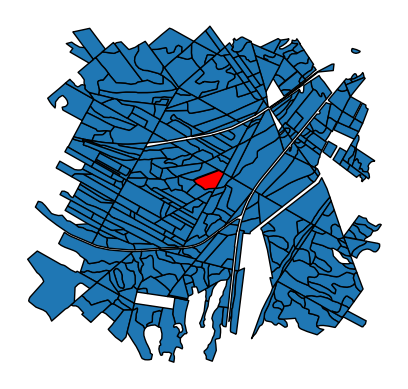
\includegraphics[width=.5\textwidth]{figures/andmestik/er_id_is10124223.png}
    \caption{Näidis ühe lageraie päringust saadud ümbrus}
    \label{fig:umbrusexample}
\end{figure}

Magistritöö peamiseks uurimisküsimuseks on, kas ja kuidas on võimalik kasutada väheste näidete (\textit{Few-Shot}) põhist alusmudelit. Selleks on aga vaja täpseid andmeid millelt õppida. Nagu eelnevalt mainitud siis metsaregistrist saadud andmed ei ole piisavalt täpsed, et neid otse kasutada. Seetõttu on vajalikud andmete täiendavat töötlemise ja maskimise etapid, kus andmed käiakse käsitsi läbi, kasutades registri andmeid maski põhjana. Ajalise piirangu tõttu pidi tegema alamvalimi. Et saada Eesti metsade kohta üldisemaid näiteid kasutati selleks KMeans klasterdamise meetodit, et jagada metsad omakorda kahte erinevasse klassi okas- ja lehtpuud. Eesmärgiks oli koguda kokku 100 raiet ja nende ümbrust, et luua piisavalt andmeid, mille pealt mudelit treenida. Kui peaks juhtuma et mõni pilt pole kõlbulik, siis valitakse samas klustrist uus lageraie piirkond.

\begin{figure}[H]
    \centering
    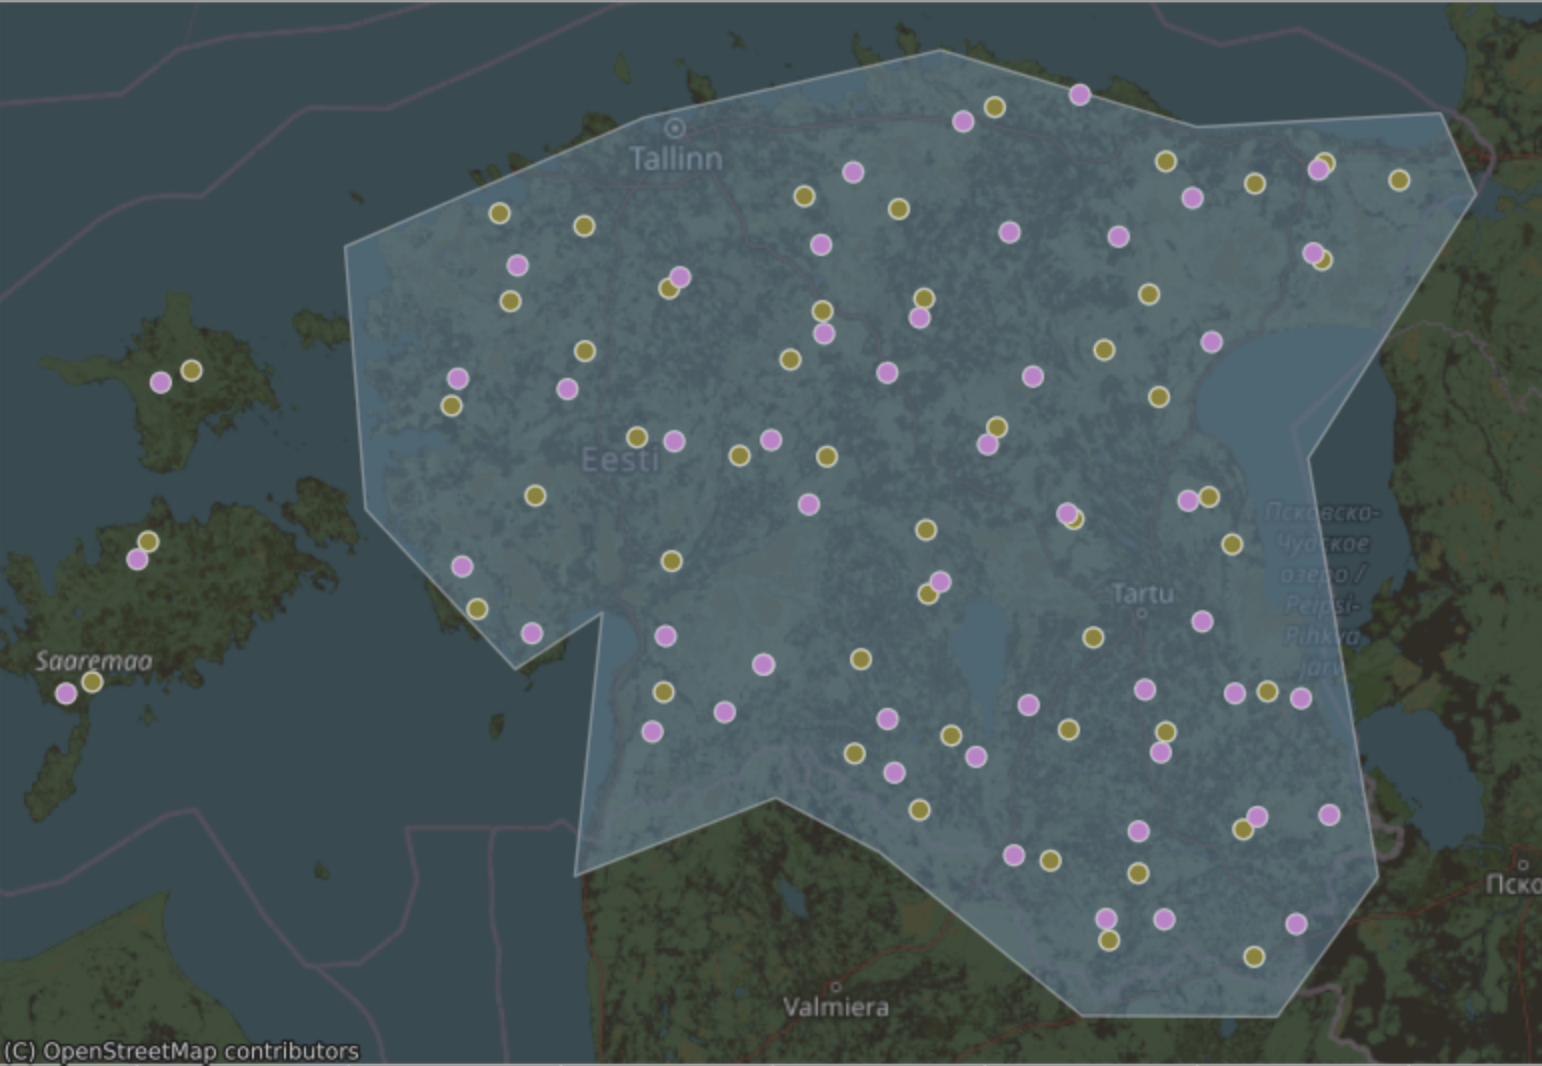
\includegraphics[width=.9\textwidth]{figures/andmestik/kmeansmap.png}
    \caption{KMeans klasterdamise tulemus, 100 raie ümbrust leht- või okaspuudega}
    \label{fig:kmeans}
\end{figure}

\begin{figure}[H]
    \centering
    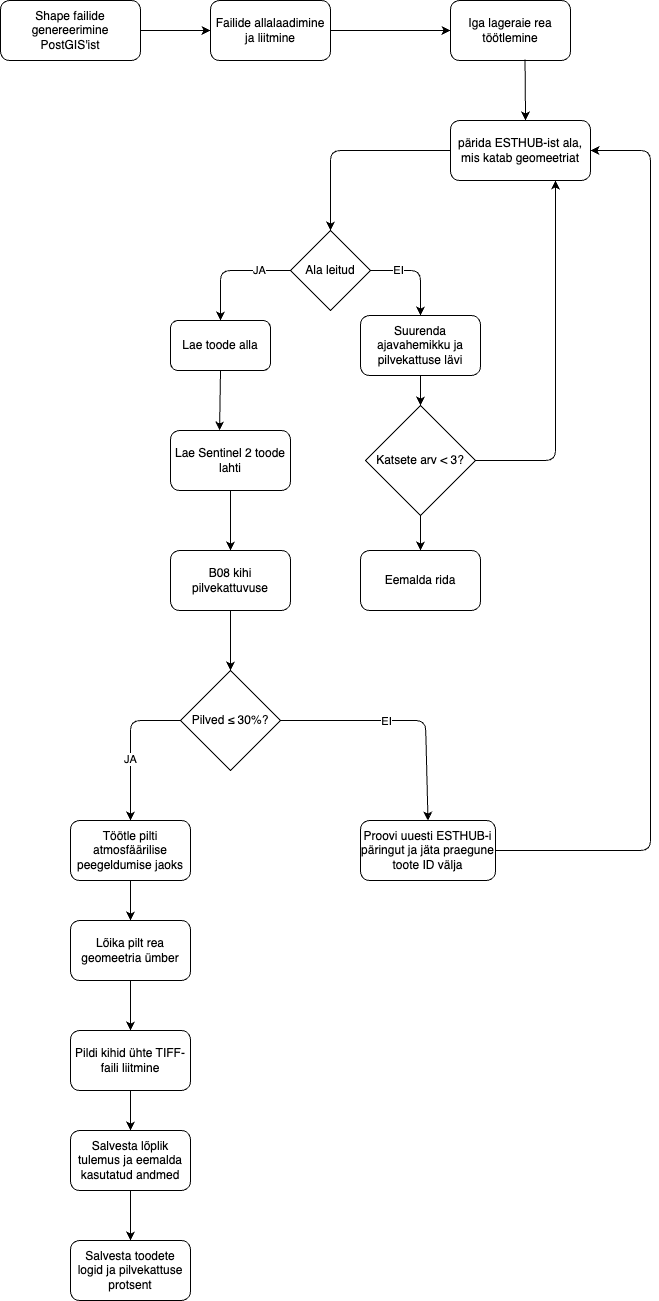
\includegraphics[width=.6\textwidth]{figures/andmestik/andmete_voog.drawio.png}
    \caption{Andmestiku loomise töövoog}
    \label{fig:terveflow}
\end{figure}

\subsection{Raie piirkonna maskide loomine}
Need sammud mis Liis teeb kui valideerib maske.